%%%%%%%%%%%%%%%%%%%%%%%%%%%%%%%%%%%%%%%%%%%%%%%%%%%%%%%%%%%%%%%%%%%%%%%%%%%%%%%
% Chapter 5 - Chronic Awake Imaging of Photothrombotic Stroke
%%%%%%%%%%%%%%%%%%%%%%%%%%%%%%%%%%%%%%%%%%%%%%%%%%%%%%%%%%%%%%%%%%%%%%%%%%%%%%%

\chapter{Chronic Awake Imaging of Photothrombotic Stroke} \label{ch:awake}

Anesthesia is widely used in preclinical neuroscience research to sedate animals while imaging despite systemic effects on neuronal and vascular function \cite{Janssen:2004ih}. The inhalation anesthetic isoflurane has been shown to reduce excitatory synaptic transmission \cite{BergJohnsen:1992wk}, impair oxygen autoregulation \cite{Aksenov:2012wh}, suppress the magnitude and speed of neurovascular coupling \cite{Pisauro:2013cx}, and cause abnormal increases in CBF \cite{Strebel:1995uh}. Isoflurane has also been shown to convey neuroprotective effects that may reduce the severity of ischemic lesions \cite{Sakai:2007wc, Burchell:2013tj} and suppress the occurrence and frequency of spreading depolarizations \cite{Kudo:2016ho}. These effects can mask the benefits of neuroprotective agents and potentially impact the outcomes of long-term studies \cite{Kapinya:ua, Seto:2014ga}. Our lab has reported \cite{Ponticorvo:2010uv, Kazmi:2013ey, Sullender:2018ff} conflicting vascular \ce{pO2} measurements that can likely be attributed to the use of different general anesthetics (urethane vs. isoflurane).

The elimination of anesthesia from neuroimaging experiments has grown increasingly popular in recent years with two primary strategies taking the forefront. The first is the usage of head-mounted microscopes that miniaturize many of the optical components into a package that can be installed on the head of a mouse \cite{Gu:1999ky, Helmchen:2001tw, Flusberg:2005tq}. While this technique allows for freely-moving tethered subjects, it requires extensive optical engineering and introduces significant motion artifacts caused by normal animal behavior \cite{Helmchen:2001tw}. Miniaturizing the system described in this dissertation would require significant sacrifices in spatial and temporal resolutions for both imaging modalities.

The second strategy involves restraining the animal's head while positioned on a rotating treadmill \cite{Pisauro:2013cx, Dombeck:2007gr, Wienisch:2011ju, Kaifosh:2013fy, Heiney:2018gq} or confined in a small chamber \cite{Silasi:2016dq}, permitting the use of existing imaging platforms. This technique allows for walking or running in place while minimizing motion of the head and imaging region. A spherical treadmill design has been used to perform awake two-photon microscopy with only an estimated 2-5 $\mu$m of lateral motion \cite{Dombeck:2007gr}, which is near the resolution of the dual-modality imaging system. This chapter details the transition from anesthetized to awake animal imaging, including the selection of a treadmill-based restraint system and \textit{in vivo} demonstrations of chronic awake imaging.



%%%%%%%%%%%%%%%%%%%%%%%%%%%%%%%%%%%%%%%%%%%%%%%%%%%%%%%%%%%%%%%%%%%%%%%%%%%%%%%
% Section 5.1 - Awake Imaging System Design
%%%%%%%%%%%%%%%%%%%%%%%%%%%%%%%%%%%%%%%%%%%%%%%%%%%%%%%%%%%%%%%%%%%%%%%%%%%%%%%
\section{Awake Imaging System Design}

The spherical treadmill described by Dombeck \textit{et al.} \cite{Dombeck:2007gr} is a popular design in the neuroscience community. It features a large (8-inch) Styrofoam ball supported on an air cushion produced by a perforated hemispheric casting. The ball allows for two dimensions of free movement, which reduces the torque the animal can apply to its permanently-attached metal headbar that encircles the cranial window. An implementation of this design using a 3D-printed base can be seen in Figure \ref{fig:awakesystems}A. A series of channels spanning the plastic cylinder direct the flow of air upwards to form the supporting air cushion. Flow is regulated using the standard house air supply and can be adjusted as needed depending on the weight of the ball and the subject. While preliminary tests showed the design was functional, the loudness of the flowing air was deemed unsuitable for practical use. The height of the entire apparatus was also a major limitation, with only the dual-modality imaging system capable of the necessary vertical translation.

% Figure - Awake System Designs
\begin{figure}
    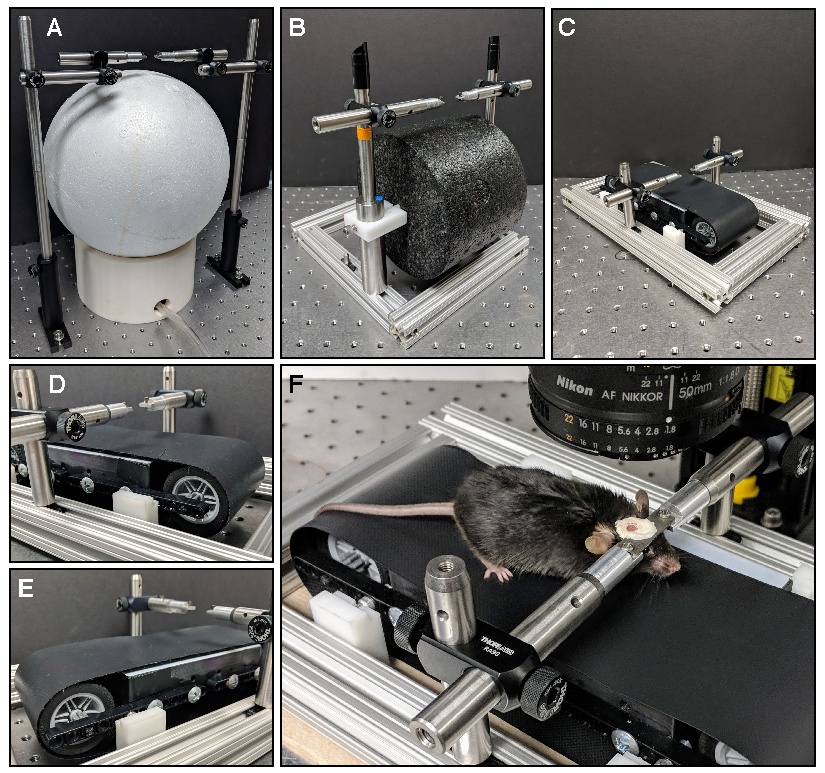
\includegraphics{figures/chapter_5/awakesystems.pdf}
    \caption{
        \label{fig:awakesystems}
        \textbf{(A)} Air-cushioned spherical treadmill, \textbf{(B)} foam wheel treadmill, and \textbf{(C)} low-profile continuous belt treadmill. Close-up of the \textbf{(D)} front and \textbf{(E)} rear pulley wheels on the belt treadmill. \textbf{(F)} Mouse head-restrained on the belt treadmill using the permanently attached headbar.
    }
\end{figure}

Two alternative designs with lower profiles were examined. The first implemented (Figure \ref{fig:awakesystems}B) a rotating foam wheel \cite{Heiney:2018gq} that allowed for one dimension of free movement. The coarse surface of the foam appeared to offer a better grip for the animal than the Styrofoam ball, making it easier to walk. While the vertical height was still substantially greater than the stereotaxic frame used during anesthetized imaging, the apparatus could easily fit under both the dual-modality and standalone MESI systems. However, issues were encountered with the stability of the rotation caused by difficulties in precisely centering the axle through the foam. These rotational variations in the position of the surface of the wheel relative to the headbar caused large motion artifacts in the resulting speckle contrast imagery despite head fixation.

The second design implemented (Figure \ref{fig:awakesystems}C) a continuous belt treadmill \cite{Royer:2012gw, Kaifosh:2013fy} that also allowed for one dimension of self-propelled movement. The rubberized tread rotated over two pulleys made from LEGO tires and axles (Figure \ref{fig:awakesystems}D-E) with the animal centered over a flat piece of plastic. This eliminated the vertical variations that negatively impacted the wheel-based design and resulted in more stable LSCI measurements when the animal moved. The height of the treadmill was also further reduced and only slightly taller than the conventional stereotaxic frame. Figure \ref{fig:awakesystems}F depicts a mouse restrained on the treadmill system via its permanently attached metal headbar (Appendix \ref{app:cranial_window}).



%%%%%%%%%%%%%%%%%%%%%%%%%%%%%%%%%%%%%%%%%%%%%%%%%%%%%%%%%%%%%%%%%%%%%%%%%%%%%%%
% Section 5.2 - Effects of Anesthesia on Hemodynamics
%%%%%%%%%%%%%%%%%%%%%%%%%%%%%%%%%%%%%%%%%%%%%%%%%%%%%%%%%%%%%%%%%%%%%%%%%%%%%%%
\section{Effects of Anesthesia on Hemodynamics}

\textit{In vivo} imaging with the head-restrained treadmill system was demonstrated by comparing awake and anesthetized hemodynamics. The subject was mounted on the treadmill using its headbar and allowed to acclimate for 10-15 minutes prior to imaging. The mounting rods were adjusted as necessary to maintain a comfortable head position and to orient the cranial window perpendicularly to the optical axis. Subjects quickly adapted to walking on the treadmill and would exhibit regularly grooming behavior when stationary.

An extended MESI acquisition was performed to monitor the stability of awake and anesthetized measurements and the transition between the two states. The awake subject was imaged continuously for one hour with a nose-cone placed directly in front of the restrained animal and delivering only medical air. General anesthesia was then quickly induced with medical-air vaporized isoflurane (2.5\%) via the nose-cone. After several minutes, the isoflurane was reduced to 1.5\% and a feedback heating pad (DC Temperature Controller, FHC) placed under the animal to regulate body temperature. The anesthetized subject was imaged for an additional one hour before being removed from anesthesia and allowed to recover on a heating pad.

% Figure - Speckle Awake vs. Anesthetized
\begin{figure}
    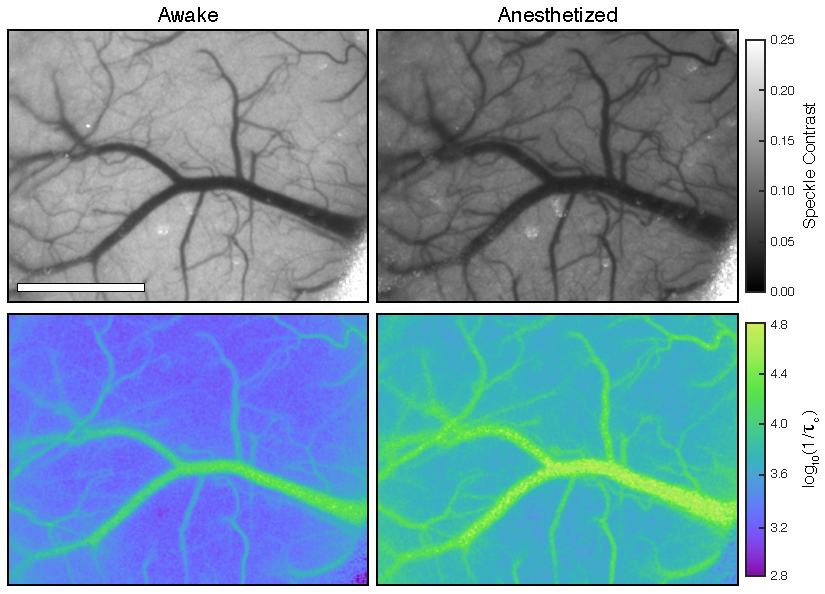
\includegraphics{figures/chapter_5/speckleawakeanes.pdf}
    \caption{
        \label{fig:speckleawakeanes}
        Speckle contrast (top) and MESI ICT (bottom) imagery from a mouse while awake (left) and anesthetized (right) exhibits the systemic change in CBF. (Scale bar = 1 mm).
    }
\end{figure}

Figure \ref{fig:speckleawakeanes} depicts averaged single-exposure (5 ms) speckle contrast images and their corresponding MESI ICT images during the awake and anesthetized states. Anesthesia caused a systematic increase in CBF as exhibited by the decrease in average speckle contrast (0.199 $\to$ 0.166) and increase in average ICT (2798 $s^{-1} \to$ 6579 $s^{-1}$). Significant vasodilation can also be seen in the large central vein and many smaller vessels only become visible in the anesthetized state. These results are consistent with volatile anesthetics being potent vasodilators that cause dose-dependent increases in baseline CBF uncoupled from local metabolic demands \cite{Masamoto:2012bj}.




%%%%%%%%%%%%%%%%%%%%%%%%%%%%%%%%%%%%%%%%%%%%%%%%%%%%%%%%%%%%%%%%%%%%%%%%%%%%%%%
% Section 5.3 - Awake Targeted Photothrombosis Induction
%%%%%%%%%%%%%%%%%%%%%%%%%%%%%%%%%%%%%%%%%%%%%%%%%%%%%%%%%%%%%%%%%%%%%%%%%%%%%%%
\section{Awake Targeted Photothrombosis Induction}

\blindtext



%%%%%%%%%%%%%%%%%%%%%%%%%%%%%%%%%%%%%%%%%%%%%%%%%%%%%%%%%%%%%%%%%%%%%%%%%%%%%%%
% Section 5.4 - Chronic Awake Post-Stroke Hemodynamics
%%%%%%%%%%%%%%%%%%%%%%%%%%%%%%%%%%%%%%%%%%%%%%%%%%%%%%%%%%%%%%%%%%%%%%%%%%%%%%%
\section{Chronic Awake Post-Stroke Hemodynamics}

\blindtext



%%%%%%%%%%%%%%%%%%%%%%%%%%%%%%%%%%%%%%%%%%%%%%%%%%%%%%%%%%%%%%%%%%%%%%%%%%%%%%%
% Section 5.5 - Discussion
%%%%%%%%%%%%%%%%%%%%%%%%%%%%%%%%%%%%%%%%%%%%%%%%%%%%%%%%%%%%%%%%%%%%%%%%%%%%%%%
\section{Discussion}

\blindtext



%%%%%%%%%%%%%%%%%%%%%%%%%%%%%%%%%%%%%%%%%%%%%%%%%%%%%%%%%%%%%%%%%%%%%%%%%%%%%%%
% END Chapter 5
%%%%%%%%%%%%%%%%%%%%%%%%%%%%%%%%%%%%%%%%%%%%%%%%%%%%%%%%%%%%%%%%%%%%%%%%%%%%%%%
